
\noindent  \textbf{Uni\'on de conjuntos.}\\
\noindent   Denotada como $A \cup B$, son todos los elementos  que pertenecen a $A$ y a $B$.
    
            \begin{center}
                $A \cup B = \lbrace x : x \in A \hspace{0.1cm} \lor \hspace{0.1cm} x \in B\rbrace$
            \end{center}

    \begin{center}
            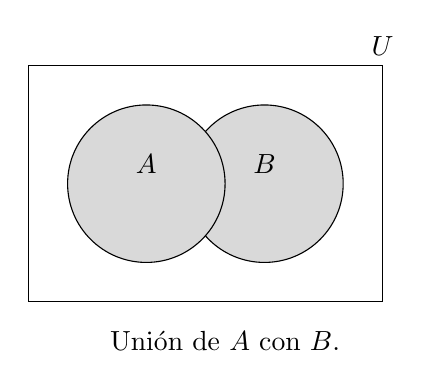
\begin{tikzpicture}
                 % Conjunto universal
                \draw[fill=white!20] (-1.5,-1.5) rectangle (3,1.5) node[above] {$U$};
                                         
                 % Conjunto B
                \draw[fill=gray!30] (1.5,0) circle (1cm) node[above] {$B$};
                
                % Conjunto A
                \draw[fill=gray!30] (0,0) circle (1cm) node[above] {$A$};
    
                % Título
                \node at (1,-2) {Uni\'on de $A$ con $B$.};
            \end{tikzpicture}
    \end{center}

\noindent \textbf{Intersección de conjuntos.}\\
\noindent  Hace referencia a todos los elementos que pertenecen tanto a $A$ como a $B$ se denota como $A \cap B$ donde,

            \begin{center}
                $A \cup B = \lbrace x : x \in A \hspace{0.1cm} \land \hspace{0.1cm} x \in B\rbrace$
            \end{center}      
        
    \begin{center}
        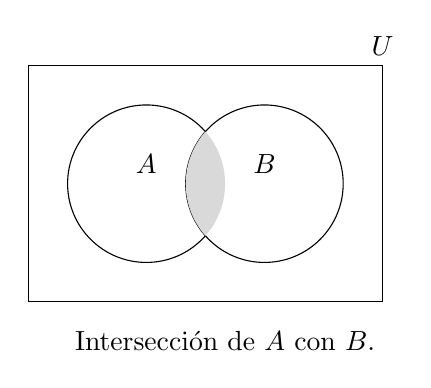
\begin{tikzpicture}  
            % Conjunto universal
            \draw[fill=white!20] (-1.5,-1.5) rectangle (3,1.5) node[above] {$U$};
             % Conjunto A
            \draw[fill=white!30] (0,0) circle (1cm) node[above] {$A$};
            % Conjunto B
            \draw[fill=white!30] (1.5,0) circle (1cm) node[above] {$B$};

            % Intersección de conjuntos
            \begin{scope}
            \clip (0,0) circle (1cm);
            \clip (1.5,0) circle (1cm);
            \fill[gray!30] (-2,-2) rectangle (4,2);
            \end{scope}
                   
            % Título
            \node at (1,-2) {Intersección de $A$ con $B$.};
        \end{tikzpicture}
     \end{center}


\noindent  \textbf{Complemento.} \\
\noindent El \textbf{complemento absoluto}, o simplemente \textbf{complemento de un conjunto} $A$, denotado por  $A^{c}$, es el conjunto de elementos que pertenecen al conjunto universo $U$ mas no al conjunto $A$.
    
    \begin{center}
            $A^{c} = \lbrace x : x \in U,  x \notin A\rbrace$
        
            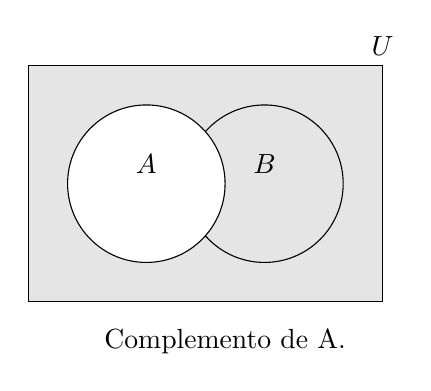
\begin{tikzpicture}                  
                % Conjunto universal
                \draw[fill=gray!20] (-1.5,-1.5) rectangle (3,1.5) node[above] {$U$};
    
                % Complemento de A
                \begin{scope}
                    \clip (0,0) circle (1cm);
                    \fill[white, opacity=0.1] (-2,-2) rectangle (2,2);
                \end{scope}
                        
                % Conjunto B
                \draw[fill=gray!20] (1.5,0) circle (1cm) node[above] {$B$};
                % Conjunto A
                \draw[fill=white!30] (0,0) circle (1cm) node[above] {$A$};
             
                % Título
                \node at (1,-2) {Complemento de A.};
            \end{tikzpicture} 
    \end{center}


\noindent \textbf{Diferencia y Diferencia sim\'etrica.}\\
\noindent La \textbf{diferencia} entre $A$ y $B$, es denotada por $A\setminus B$, es el conjunto de elementos que pertenecen a $A$ mas no pertenecen a $B$, es decir:
    
    \begin{center}
            $A \setminus  B = \lbrace x : x \in A  \hspace{0.1cm} \lor \hspace{0.1cm} x \notin B\rbrace$
            
    
            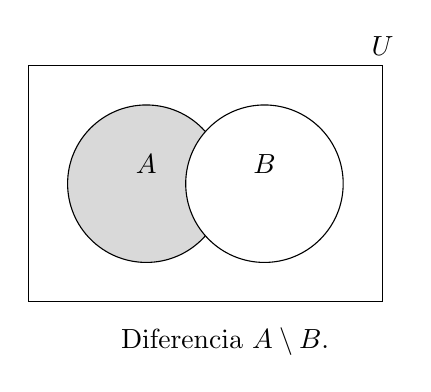
\begin{tikzpicture}
                 % Conjunto universal
                \draw[fill=white!20] (-1.5,-1.5) rectangle (3,1.5) node[above] {$U$};

                % Conjunto A
                \draw[fill=gray!30] (0,0) circle (1cm) node[above] {$A$};
                
                 % Conjunto B
                \draw[fill=white!30] (1.5,0) circle (1cm) node[above] {$B$};
                
    
                % Título
                \node at (1,-2) {Diferencia $A \setminus B$.};
            \end{tikzpicture}

    \end{center}

\noindent \textbf{Diferencia y Diferencia sim\'etrica.}\\
\noindent  La \textbf{diferencia sim\'etrica} de dos conjutnos $A$ y $B$, denotada como $A \oplus B$, consiste en los elementos que pertenecen a $A$ \'o a $B$ mas no a los elementos que pertenecen a ambos $A$ y $B$, esto es:

        \begin{center}
            $A \oplus B = (A \cup B)\setminus(A \cap B)$ \hspace{1cm} \'o \hspace{1cm} $A \oplus B = (A \setminus B)\cup (B^{'} \setminus A)$\vspace{15px} \\
              

            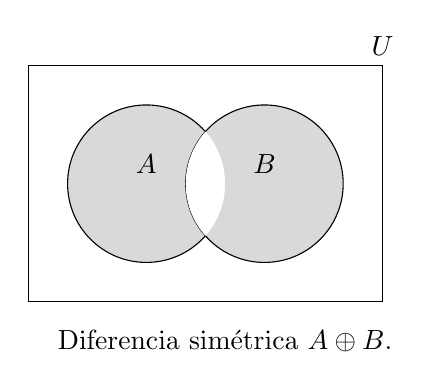
\begin{tikzpicture}  
            % Conjunto universal
            \draw[fill=white!20] (-1.5,-1.5) rectangle (3,1.5) node[above] {$U$};
             % Conjunto A
            \draw[fill=gray!30] (0,0) circle (1cm) node[above] {$A$};
            % Conjunto B
            \draw[fill=gray!30] (1.5,0) circle (1cm) node[above] {$B$};

            % Intersección de conjuntos
            \begin{scope}
            \clip (0,0) circle (1cm);
            \clip (1.5,0) circle (1cm);
            \fill[white!30] (-2,-2) rectangle (4,2);
            \end{scope}
                   
            % Título
            \node at (1,-2) {Diferencia sim\'etrica $A \oplus B$.};
            \end{tikzpicture}
    \end{center}